\documentclass[a4paper,12pt]{article}

\usepackage{mystyle}

\graphicspath{ {images/} }


% https://tex.stackexchange.com/questions/5461/is-it-possible-to-change-the-size-of-an-arrowhead-in-tikz-pgf
\usetikzlibrary{arrows.meta}

% https://tex.stackexchange.com/questions/261591/arrow-above-text-like-widehat
\usepackage{esvect}

% https://tex.stackexchange.com/questions/32501/how-to-get-a-good-divisible-by-symbol
\DeclareRobustCommand{\divby}{%
  \mathrel{\vbox{\baselineskip.65ex\lineskiplimit0pt\hbox{.}\hbox{.}\hbox{.}}}%
}


\definecolor{light-cyan}{RGB}{0, 204, 204}
\definecolor{light-purple}{RGB}{138, 43, 226}


\author{Алексеев Василий}
\title{Семинар 2}
\date{8 + 14 сентября 2020}


\begin{document}
  \maketitle
  
  \tableofcontents

  \thispagestyle{empty}
  
  \newpage
  
  \pagenumbering{arabic}


  \section{Вектора (-ы?)}
  
  Вектор~---~направленный отрезок (\ref{fig:vector}).
  Вектор можно обозначать одной строчной буквой, например $\bds a$, или двумя: началом и концом, например $\vv{AB}$.
  
  \begin{figure}[h]
    \centering
    
    \begin{tikzpicture}
      \draw[-{Latex[length=5mm, width=2mm]}, thick] (0,0) node[anchor=north west]{$A$} -- (5,5) node[anchor=north west]{$B$};
      \draw[ultra thick, fill] (0,0) circle[radius=0.05];
    \end{tikzpicture}
    
    \caption{Вектор характеризуется направлением и величиной.}
    \label{fig:vector}
  \end{figure}
  
  \begin{definition}[Коллинеарность]
    Два ненулевых вектора $\bds a$ и $\bds b$ называются \emph{коллинеарными}, если существует прямая, которой они параллельны (\ref{fig:collinearity}).
    Коллинеарность обозначается $\bds a \hm\parallel \bds b$.
    Если при этом $\bds a$ и $\bds b$ направлены в одну сторону, то можно писать $\bds a \hm\upuparrows \bds b$,
    если в разные стороны~---~$\bds a \hm\updownarrows \bds b$.
    Нулевой вектор коллинеарен любому вектору.
  \end{definition}
  
  \begin{figure}[h]
    \centering
    
    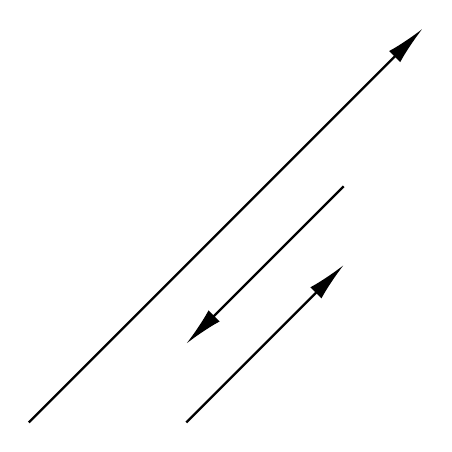
\begin{tikzpicture}
      \draw[-{Latex[length=5mm, width=2mm]}, thick] (0,0) -- (5,5);
      \draw[{Latex[length=5mm, width=2mm]}-, thick] (2,1) -- (4,3);
      \draw[-{Latex[length=5mm, width=2mm]}, thick] (2,0) -- (4,2);
    \end{tikzpicture}
    
    \caption{Коллинеарные вектора.}
    \label{fig:collinearity}
  \end{figure}
  
  \begin{definition}[Компланарность]
    Три ненулевых вектора $\bds a$, $\bds b$ и $\bds c$ называются \emph{компланарными}, если существует плоскость, которой они параллельны (\ref{fig:coplanarity}).
    Три вектора, два из которых ненулевые, а третий нулевой, всегда компланарны.
  \end{definition}
  
  \begin{figure}[h]
    \centering
    
    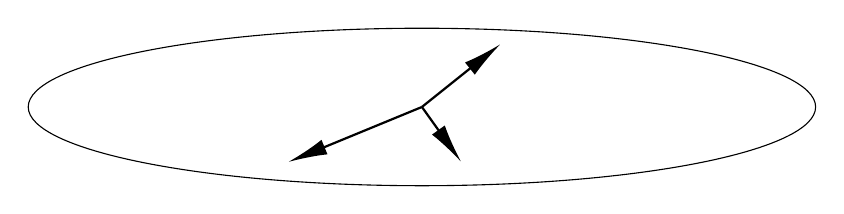
\begin{tikzpicture}
      \draw (0,0) ellipse (5cm and 1cm);
      \draw[-{Latex[length=5mm, width=2mm]}, thick] (0,0) -- (1,0.8);
      \draw[-{Latex[length=5mm, width=2mm]}, thick] (0,0) -- (0.5,-0.7);
      \draw[-{Latex[length=5mm, width=2mm]}, thick] (0,0) -- (-1.7,-0.7);
    \end{tikzpicture}
    
    \caption{Компланарные вектора.}
    \label{fig:coplanarity}
  \end{figure}
  
  \begin{definition}[Равенство векторов]
    Будем считать два вектора $\bds a$ и $\bds b$ равными, если они
    \begin{itemize}
      \item равны по длине $|\bds a| = |\bds b|$
      \item коллинеарны $\bds a \parallel \bds b$
      \item одинаково направлены $\bds a \upuparrows \bds b$
    \end{itemize}
    Точка приложения при равенстве не учитывается\footnote{То есть получается, что можно нарисовать несколько несовпадающих, но равных векторов. Хотя в зависимости от конкретной задачи может быть важным различать векторы с разной точкой приложения. Например, в физике, при действии сил на тело.}.
  \end{definition}
  
  На множестве векторов определены следующие операции:
  \begin{itemize}
    \item Сложение векторов:
      \[
        \vv{AB} + \vv{BC} = \vv{AC}
      \]
    \item Умножение вектора $\bds a$ на число $\alpha \in \RR$.
      Результирующий вектор обозначается как $\alpha \bds a$ и определяется свойствами:
      \[
        \left\{
          \begin{aligned}
            &|\alpha \bds a| = |\alpha| \cdot |\bds a|\\
            &\alpha \bds a \parallel \bds a\\
            &\left\{
               \begin{aligned}
                 &\alpha \bds a \upuparrows \bds a, \alpha > 0\\
                 &\alpha \bds a \updownarrows \bds a, \alpha < 0
               \end{aligned}
             \right.
          \end{aligned}
        \right.
      \]
  \end{itemize}
  
  Множество векторов в $\RR^3$ с введёнными операциями сложения и умножения на число из $\RR$ образуют линейное пространство.
  Но рассмотрим векторы на одной прямой: сложение и умножение на число не выводят с прямой.
  То же самое с векторами на плоскости: сложение и умножение на число даёт вектор, также лежащий в той же плоскости.
  Таким образом, не только векторы из всего $\RR^3$ образуют линейное пространство, но и векторы, параллельные одной прямой, и векторы, параллельные одной плоскости.
  Множество векторов из одного нулевого вектора также образуют линейное пространство.
  Таким образом,
  \begin{itemize}
    \item нульмерное векторное пространство~---~нулевой вектор
    \item одномерное векторное пространство
      \[
        \{\bds v \in \RR^3 \mid \bds v \parallel l\}, \quad \mbox{$l$~---~прямая}
      \]
    \item двумерное векторное пространство
      \[
        \{\bds v \in \RR^3 \mid \bds v \parallel \alpha\}, \quad \mbox{$\alpha$~---~плоскость}
      \]
    \item трёхмерное векторное пространство~---~$\RR^3$
  \end{itemize}
  
  \begin{definition}
    Линейная комбинация векторов $\bds a_1, \ldots, \bds a_n$:
    \[
      \alpha_1 \bds a_1 + \ldots + \alpha_n \bds a_n, \quad \alpha_i \in \RR, 1 \leq i \leq n
    \]
    
    Нетривиальная линейная комбинация~---~когда хотя бы один их коэффициентов $\alpha_i$ отличен от нуля:
    $\sum\limits_{i=1}^n \alpha_i^2 \hm> 0$.
  \end{definition}
  
  \begin{definition}[Линейно зависимая система векторов]
    Система векторов $\bds a_1, \ldots, \bds a_n$ называется линейно зависимой, если существует их нетривиальная линейная комбинация, равная нулевому вектору:
    \[
      \left\{
        \begin{aligned}
          &\alpha_1 \bds a_1 + \ldots + \alpha_n \bds a_n = \bds 0\\
          &\alpha_1^2 + \ldots + \alpha_n^2 > 0
        \end{aligned}
      \right.
    \]
  \end{definition}
  
  \begin{example}
    Система из одного нулевого вектора линейно зависима.
  \end{example}
  
  \begin{theorem}
    Система из $k > 1$ вектора линейно зависима тогда и только тогда, когда один из векторов системы представим как линейная комбинация остальных.
  \end{theorem}
  
  \begin{proof}
    Пусть $\bds a_1, \ldots, \bds a_n$~---~линейно зависимы.
    Это значит, что
    \[
      \alpha_1 \bds a_1 + \ldots + \alpha_n \bds a_n = \bds 0
    \]
    и некоторый $\alpha_j \hm{\not=} 0$.
    Поэтому
    \[
      \alpha_j = \sum\limits_{\substack{1 \leq i \leq n\\i \not= j}} -\frac{\alpha_i}{\alpha_j} \bds a_i
    \]
    
    И наоборот, пусть некоторый $\bds a_j$ представим как линейная комбинация остальных векторов из набора с коэффициентами $\alpha_i'$:
    \[
      \bds a_j = \sum\limits_{\substack{1 \leq i \leq n\\i \not= j}} \alpha_i' \bds a_i
    \]
    Тогда
    \[
      \alpha_1' \bds a_1 + \ldots + (-1) \cdot \bds a_j + \ldots + \alpha_n' \bds a_n = \bds 0
    \]
    и по крайней мере один коэффициент $-1$ при разложении нуля $\bds 0$ в линейную комбинацию векторов $\{\bds a_i\}_{i=1}^n$ не равен нулю.
  \end{proof}
  
  \begin{theorem}\label{theo:linear-dependence-criteria}
    Критерии линейной зависимости систем векторов:
    \begin{itemize}
      \item Один вектор линейно зависим $\Leftrightarrow$ это нулевой вектор.
      \item Два вектора линейно зависимы $\Leftrightarrow$ эти векторы коллинеарны.
      \item Три ветора линейно зависимы $\Leftrightarrow$ эти векторы компланарны.
      \item Любые четыре вектора линейно зависимы\footnote{В $\RR^3$.}.
    \end{itemize}
  \end{theorem}
  
  \begin{definition}[Базис]
    Базисом в пространстве называется
    \begin{itemize}
      \item упорядоченная
      \item линейно независимая
      \item полная\footnote{Любой вектор пространства может быть разложен по системе.}
    \end{itemize}
    система векторов.
  \end{definition}
  
  Из теоремы (\ref{theo:linear-dependence-criteria}) следует, что
  \begin{itemize}
    \item В нулевом пространстве не существует базиса.
    \item В одномерном пространстве ненулевой вектор образует базис.
    \item В двумерном пространстве пара неколлинеарных векторов образует базис.
    \item В трёхмерном пространстве тройка некомпланарных векторов образует базис.
  \end{itemize}
  
  \begin{remark}
    При заданном базисе $\{\bds e_1, \ldots, \bds e_n\}$ каждому вектору можно поставить в соответствие набор чисел~---~коэффициентов при разложении вектора по базису $\bds a \hm= \alpha_1 \bds e_1 \hm+ \ldots \hm+ \alpha_n \bds e_n$:
    \[
        \bds a \leftrightarrow (\alpha_1, \ldots, \alpha_n) \in \RR^n
    \]
    Соответствие взаимно однозначное, потому что базисная система векторов линейно независима.
  \end{remark}
  
  \begin{remark}[Про матричное умножение]
    Почему матричное умножение введено именно так: $C_{m\times n} \hm= A_{m\times p}B_{p\times n}$, $c_{ij} \hm= \sum\limits_{k=1}^p a_{ik} b_{kn},\ 1 \hm\leq i \hm\leq m, 1 \hm\leq j \hm\leq n$?
    
    Пусть есть ортонормированный\footnote{Вектора взаимно перпендикулярны и по длине равны единице $1$.} базис $\bds e_1, \bds e_2$.
    Повернём вектор $\bds v$ с компонентами $(1, 0)$ на угол $45$ градусов против часовой стрелки (\ref{fig:turning-vector}).
    
    \begin{figure}[h]
      \centering
      
      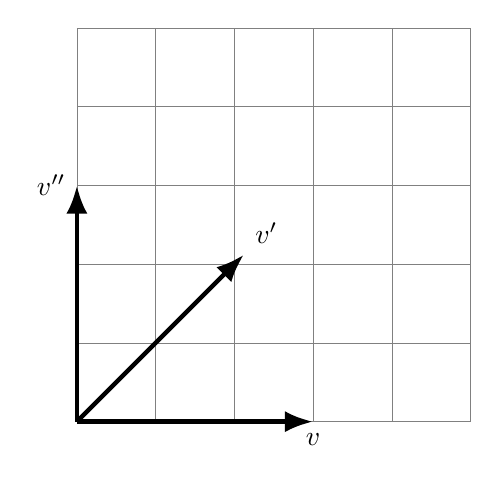
\begin{tikzpicture}
        \draw[step=1cm,gray,very thin] (0,0) grid (5,5);
        \draw[-Latex,ultra thick] (0,0) -- (3,0) node[anchor=north]{$\boldsymbol{v}$};
        \draw[-Latex,ultra thick] (0,0) -- (2.121,2.121) node[anchor=south west]{$\boldsymbol{v'}$};
        \draw[-Latex,ultra thick] (0,0) -- (0,3) node[anchor=east]{$\boldsymbol{v''}$};
      \end{tikzpicture}
      
      \caption{Несколько поворотов вектора $\bds v$ на $45$ градусов против часовой стрелки.}
      \label{fig:turning-vector}
    \end{figure}
    
    Получим вектор $\left(1/\sqrt{2}, 1/\sqrt{2}\right)$.
    Проверим, что матрица $\left(\begin{smallmatrix}1/\sqrt{2} & -1/\sqrt{2}\\ 1/\sqrt{2} & 1/\sqrt{2}\end{smallmatrix}\right)$ как раз задаёт нужное преобразование:
    \[
      v'
      = A \bds v
      = \begin{pmatrix}
          1/\sqrt{2} & -1/\sqrt{2}\\
          1/\sqrt{2} & 1/\sqrt{2}
        \end{pmatrix}
        \begin{pmatrix}
          1 \\ 0
        \end{pmatrix}
      = \begin{pmatrix}
          1/\sqrt{2} \\ 1/\sqrt{2}
        \end{pmatrix}
    \]
    
    Снова повернём вектор на угол $45$ градусов против часовой стрелки.
    Должны получить вектор с компонентами $\left(\begin{smallmatrix}0 \\ 1\end{smallmatrix}\right)$:
    \[
      v''
      = A \bds v'
      = \begin{pmatrix}
          1/\sqrt{2} & -1/\sqrt{2}\\
          1/\sqrt{2} & 1/\sqrt{2}
        \end{pmatrix}
        \begin{pmatrix}
          1/\sqrt{2} \\ 1/\sqrt{2}
        \end{pmatrix}
      = \begin{pmatrix}
          0 \\ 1
        \end{pmatrix}
    \]
    
    Какой матрицей задаётся поворот сразу на $90$ градусов против часовой стрелки?
    Как из вектора
    $\left(\begin{smallmatrix}1 \\ 0\end{smallmatrix}\right)$
    сразу получить вектор
    $\left(\begin{smallmatrix}0 \\ 1\end{smallmatrix}\right)$?
    
    Возведём матрицу, задающую поворот на $45$ против часовой стрелки, в квадрат:
    \[
      A^2
      = A A
      = \begin{pmatrix}
          1/\sqrt{2} & -1/\sqrt{2}\\
          1/\sqrt{2} & 1/\sqrt{2}
        \end{pmatrix}
        \begin{pmatrix}
          1/\sqrt{2} & -1/\sqrt{2}\\
          1/\sqrt{2} & 1/\sqrt{2}
        \end{pmatrix}
      = \begin{pmatrix}
          0 & -1\\
          1 & 0
        \end{pmatrix}
    \]
    и умножим её на исходный вектор $\bds v$:
    \[
      A^2 \bds v
      = \begin{pmatrix}
          0 & -1\\
          1 & 0
        \end{pmatrix}
        \begin{pmatrix}
          1 \\ 0
        \end{pmatrix}
      = \begin{pmatrix}
          0 \\ 1
        \end{pmatrix}
    \]
    
    Таким образом, благодаря введённому матричному умножению, матрица композиции линейных преобразований получилась равна произведению матриц этих преобразований.
  \end{remark}
  
  \begin{definition}[Система координат]
    Декартовой системой координат\footnote{Помимо декартовой, есть и другие системы координат. Например полярная, когда положение точки на плоскости определяется по расстоянию $r$ от начала координат $O$ и по углу $\phi$, которое направление из начала координат на точку образует с выбранным направлением $\bds l$: $\bds a \hm\leftrightarrow (r, \phi)$.} называется совокупность точки и базиса $O; \bds e_1, \ldots, \bds e_n$.
    Точка $O$ называется началом отчёта.
  \end{definition}
  
  \begin{remark}
    При заданной системе координат $O; \bds e_1, \ldots, \bds e_n$ каждой точке $A$ можно поставить в соответствие набор чисел~---~компонент радиуса-вектора точки в базисе $\vv{OA} \hm= \alpha_1 \bds a_1 \hm+ \ldots \hm+ \alpha_n \bds a_n$:
    \[
      A \leftrightarrow (\alpha_1, \ldots, \alpha_n) \in \RR^n
    \]
  \end{remark}
  
  
  \begin{problem}[1.6]
    $\bds a(-5, -1), \bds b(-1, 3)$~---~проверить, что базис.
    Разложить $\bds c(-1, 2)$ и $\bds d(2, -6)$ по этому базису.
  \end{problem}
  
  \begin{solution}
    Для доказательства того, что $\bds a$ и $\bds b$ вместе образуют базис, достаточно проверить их линейную независимость:
    \[
      \begin{vmatrix}
        -5 & -1\\
        -1 & 3
      \end{vmatrix}
      = -15 - 1
      = -16
      \not= 0
    \]
    
    Теперь разложим, например, вектор $\bds c$ по $\bds a$ и $\bds b$ (с вектором $\bds d$ будет аналогично):
    \[
      \bds c = \alpha \bds a + \beta \bds b
    \]
    \[
      \begin{pmatrix}
        -1 \\ 2
      \end{pmatrix}
      = \alpha \begin{pmatrix}
          -5 \\ -1
        \end{pmatrix}
        + \beta \begin{pmatrix}
          -1 \\ 3
        \end{pmatrix}
      = \begin{pmatrix}
          -5\alpha - \beta\\
          -\alpha + 3\beta
        \end{pmatrix}
      = \begin{pmatrix}
          -5 -1\\
          -1 + 3
        \end{pmatrix}
        \begin{pmatrix}
          \alpha \\ \beta
        \end{pmatrix}
    \]
    
    Решаем получившуюся систему методом Крамера:
    \[
      \Delta = \begin{vmatrix}
        -5 & -1\\
        -1 & 3
      \end{vmatrix} = -16
    \]
    \[
      \Delta_1 = \begin{vmatrix}
        -1 & -1\\
        -2 & 3
      \end{vmatrix} = -1
    \]
    \[
      \Delta_2 = \begin{vmatrix}
        -5 & -1\\
        -1 & 2
      \end{vmatrix} = -11
    \]
    
    И коэффициенты разложения:
    \[
      \left\{
        \begin{aligned}
          &\alpha = \frac{\Delta_1}{\Delta} = \frac{1}{16}\\
          &\beta = \frac{\Delta_2}{\Delta} = \frac{11}{16}
        \end{aligned}
      \right.
    \]
  \end{solution}
  

  \begin{problem}[1.11(1)]
    Компланарны ли $\bds l, \bds m, \bds n$?
    \[
      \left\{
        \begin{aligned}
          &\bds l = 2 \bds a - \bds b - \bds c\\
          &\bds m = 2 \bds b - \bds c - \bds a\\
          &\bds n = 2 \bds c - \bds a - \bds b
        \end{aligned}
      \right.
    \]
    (векторы $\bds a, \bds b, \bds c$ некомпланарны).
  \end{problem}
  
  \begin{solution}
    Векторы $\bds a, \bds b, \bds c$ некомпланарны $\Rightarrow$ образуют базис.
    Компланарность $\bds l, \bds m, \bds n$ $\Leftrightarrow$
    линейная зависимость $\bds l, \bds m, \bds n$.
    Для проверки линейной зависимости или независимости можно посчитать определитель матрицы, составленной из компонент векторов $\bds l, \bds m, \bds n$ в базисе $\bds a, \bds b, \bds c$ (столбец матрицы~---~компоненты в разложении по данному вектору базиса):
    \[
      \begin{vmatrix}
        2 & -1 & -1\\
        -1 & 2 & -1\\
        -1 & -1 & 2
      \end{vmatrix}
      \stackrel{(2) = (2) + (3)}{=} \begin{vmatrix}
        2 & -1 & -1\\
        -2 & 1 & 1\\
        -1 & -1 & 2
      \end{vmatrix}
    \]
    
    Откуда видно, что $(1) = -\bigl((2) + (3)\bigr)$, или, если от строчек вернуться к векторам:
    \[
      \bds l = -(\bds m + \bds n) = -\bds m - \bds n
    \]
    \[
      \bds l + \bds m + \bds n = 0
    \]
  \end{solution}
  
  
  \begin{problem}[1.24(1)]
    Три точки, не лежащие на одной прямой: $O, A, B$.
    Векторы $\vv{OA}, \vv{OB}$~---~базис.
    Найти вектор $\vv{OM}$, где $M \hm\in [AB]$, так что $|AM| \hm\div |MB| \hm= m \hm\div n$.
  \end{problem}
  
  \begin{solution}
    \[
      \vv{OM} = \vv{OA} + \vv{AM}
    \]
    \[
      \vv{AM} = \frac{m}{m + n} \vv{AB} = \frac{m}{m + n} \bigl(\vv{OB} - \vv{OA} \bigr)
    \]
    \[
      \vv{OM} = \frac{n}{m + n} \vv{OA} + \frac{m}{m + n} \vv{OB} = \left(\frac{n}{m + n}, \frac{m}{m + n}\right)
    \]
  \end{solution}
  
  
  \begin{problem}[1.51]
    Доказать, что три отрезка, соединяющие середины скрещивающихся рёбер тетраэдра, пересекаются в одной точке и делятся этой точкой пополам.
  \end{problem}

  \begin{solution}
    Пусть $P, Q, R, H$~---~середины соответственных рёбер тетраэдра (см. рисунок \ref{fig:tetrahedron}).
    Тогда $PH \hm\parallel SB$ как средняя линия в $\triangle ASB$ и $QR \hm\parallel SB$ как средняя линия в $\triangle CBS$.
    Поэтому $PH \hm\parallel QR$.
    Аналогично $PQ \hm\parallel HR$.
    Значит, $PQRH$~---~параллелограмм, и точка пересечения диагоналей $O \hm= PR \hm\cap HQ$ делит их пополам.
    
    Аналогично рассматривается случай с ещё одним отрезком, соединяющим середины $SB$ и $AC$ (он рассматривается в паре с уже упомянутым отрезком $PR$ или $HQ$: они~---~диагонали в другом параллелограмме, ...). Точка их пересечения совпадёт с $O$, потому что у $PR$ (или у $HQ$) всего одна середина.
    
    Итого, все три интересующих отрезка пересекаются в одной точке и делятся ей пополам.
    
    \begin{figure}[h]
      \centering
      
      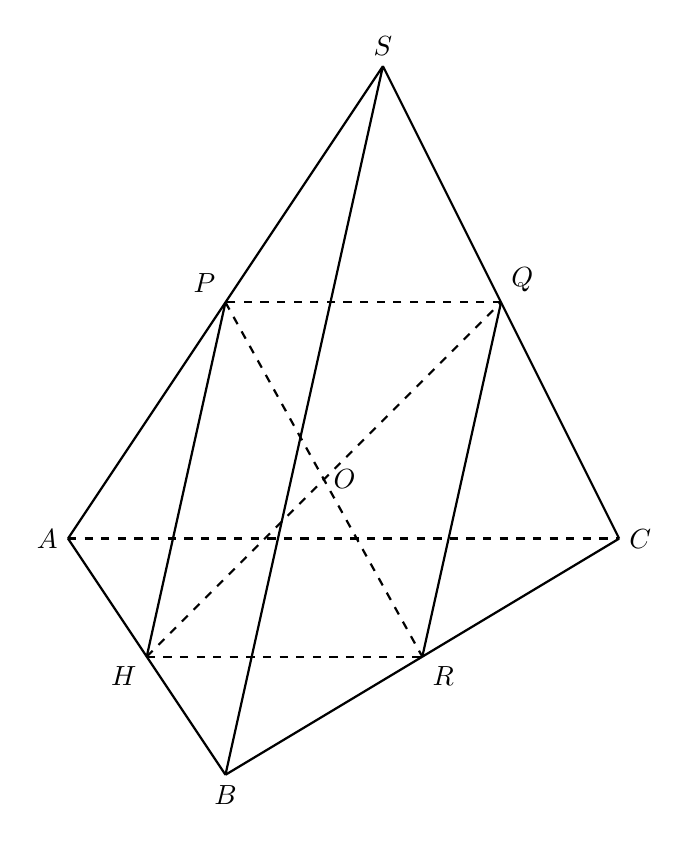
\begin{tikzpicture}
        \draw[-, thick] (2,0) node[anchor=north]{$B$} -- (7,3) node[anchor=west]{$C$}
                        (7,3)                         -- (4,9) node[anchor=south]{$S$}
                        (4,9)                         -- (0,3) node[anchor=east]{$A$}
                        (0,3)                         -- (2,0)
                        (2,0)                         -- (4,9);
        \draw[dashed, thick] (0,3) -- (7,3);
        \draw[dashed, thick] (5.5,6) node[anchor=south west]{$Q$} -- (2,6)     node[anchor=south east]{$P$}
                             (1,1.5) node[anchor=north east]{$H$} -- (4.5,1.5) node[anchor=north west]{$R$};
        \draw[-, thick] (4.5,1.5) -- (5.5,6)
                        (2,6) -- (1,1.5);
        \draw[dashed, thick] (2,6) -- (4.5,1.5)
                             (1,1.5) -- (5.5,6);
        \node[anchor=west] at (3.25,3.75) {$O$};
        %\draw[ultra thick, fill] (0,0) circle[radius=0.05];
      \end{tikzpicture}
      
      \caption{Середины четырёх рёбер тетраэдра.}
      \label{fig:tetrahedron}
    \end{figure}
  \end{solution}
  
  
  \begin{problem}[1.39]
    Однородная проволока~---~угол $AOB$.
    При этом $|OA| \hm= a$, $|OB| \hm= b$.
    Найти координаты центра тяжести проволоки в системе координат: $O, \vv{OA}/a, \vv{OB}/b$.
  \end{problem}
  
  \begin{solution}
    Обозначим за $\rho$ плотность проволоки на единицу длины.
    Пусть также $\bds e_1 \hm\equiv \vv{OA}/a$ и $\bds e_2 \hm\equiv \vv{OB}/B$.
    Тогда радиус-вектор центра масс:
    \[
      \bds r_c
      = \frac{\sum\nolimits_i m \bds r_i}{\sum\nolimits_i m_i}
      = \frac{(\rho \cdot a) \cdot (a/2 \cdot \bds e_1) + (\rho \cdot b) \cdot (b/2 \cdot \bds e_2)}{\rho \cdot a + \rho \cdot b}
      = \frac{1}{2(a + b)} \Bigl(a^2 \bds e_1 + b^2 \bds e_2\Bigr)
    \]
  \end{solution}
  
  
  \begin{problem}[1.37]
    В плоскости треугольника $ABC$ найти точку $O$, такую что
    \[
      \vv{OA} + \vv{OB} + \vv{OC} = \bds 0
    \]
    
    Есть ли ещё такие точки?
  \end{problem}
  
  \begin{solution}
    \par\indent
    
    \emph{Вспомогательная часть $1$: координаты центра масс треугольника.}
    
    \[
      \bds r_c(\triangle ABC) = \frac{1}{3} \bigl(\bds r_A + \bds r_B + \bds r_C\bigr)
    \]
    
    \medskip
    
    \emph{Вспомогательная часть $2$: координаты точки пересечения медиан треугольника.}
    
    Пусть $AM$~---~медиана, проведённая из вершины $A$ треугольника к стороне $BC$ (\ref{fig:intersecting-medians}).
    
    \begin{figure}[h]
      \centering
      
      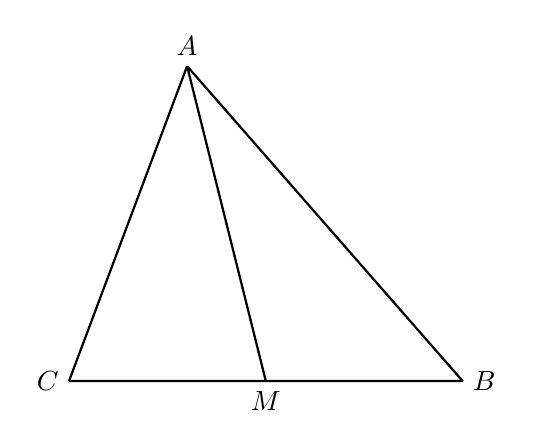
\begin{tikzpicture}
        \draw[-,thick] (0,0) node[anchor=east]{$C$} -- (5,0) node[anchor=west]{$B$}
                       (5,0)                        -- (1.5,4) node[anchor=south]{$A$}
                       (1.5,4)                      -- (0,0)
                       (1.5,4)                      -- (2.5,0) node[anchor=north]{$M$};
      \end{tikzpicture}
      
      \caption{Медиана $AM$ в треугольнике $ABC$.}
      \label{fig:intersecting-medians}
    \end{figure}
 
    Радиус-вектор точки $M$:
    \[
      \bds r_{M} = \bds r_C + \vv{CM} = \bds r_C + \frac{1}{2} \vv{CB}
      = \bds r_C + \frac{1}{2} \bigl(\bds r_B - \bds r_C\bigr)
      = \frac{1}{2} \bigl(\bds r_B + \bds r_C\bigr)
    \]
    
    Вектор $\vv{AM}$:
    \[
      \vv{AM} = \bds r_{M} - \bds r_A
      = \frac{1}{2} \bigl(\bds r_B + \bds r_C\bigr) - \bds r_A
      = \frac{1}{2} \bigl(\bds r_B + \bds r_C - 2 \bds r_A\bigr)
    \]
    
    Обозначим точкой $Q$ центр масс.
    Вектор $\vv{AQ}$:
    \[
      \vv{AQ} = \bds r_c - \bds r_A
      = \frac{1}{3} \bigl(\bds r_A + \bds r_B + \bds r_C\bigr) - \bds r_A
      = \frac{1}{3} \bigl(\bds r_B + \bds r_C - 2 \bds r_A\bigr)
    \]
    
    Получаем, что $\vv{AQ} \hm\upuparrows \vv{AM}$, причём $|AQ| \hm\div |AM| \hm= 2 \hm\div 3$.
    Значит, $Q \hm\in [AM]$.
    
    Аналогично доказывается, что $Q$ лежит на медианах из вершин $B$ и $C$.
    Так как несовпадающие прямые могут иметь не больше одной общей точки, то получаем, что точка пересечения медиан треугольника совпадает с его центром масс.
    
    \medskip
    
    \emph{Собственно решение задачи.}
    
    \[
      \vv{AB} + \vv{AC}
      = \overbrace{\left(\vv{AO} + \vv{OA}\right)}^{\bds 0} + \left(\vv{AO} + \vv{OB}\right) + \left(\vv{AO} + \vv{OC}\right)
      = 3 \vv{AO} + \left(\vv{OA} + \vv{OB} + \vv{OC}\right)
      = 3 \vv{AO}
    \]
    
    То есть
    \[
      \vv{AO} = \frac{1}{3} \left(\vv{AB} + \vv{AC}\right)
    \]
    
    Или, если переписать через радиус-векторы:
    \[
      \bds r_O - \bds r_A = \frac{1}{3} (\bds r_B - \bds r_A + \bds r_C - \bds r_A)
    \]
    
    Откуда получаем выражение для $\bds r_O$:
    \[
      \bds r_O = \frac{1}{3} (\bds r_A + \bds r_B + \bds r_C)
    \]
    
    Что значит, что точка $O$~---~точка пересечения медиан $\triangle ABC$.
    
    Существует ли ещё одна точка $Q \hm{\not=} O$, такая что $\vv{QA} \hm+ \vv{QB} \hm+ \vv{QC} \hm= \bds 0$?
    Допустим, такая точка $Q$ существует.
    Тогда
    \[
      \left\{
        \begin{aligned}
          &\vv{QO} = \vv{QA} + \vv{AO}\\
          &\vv{QO} = \vv{QB} + \vv{BO}\\
          &\vv{QO} = \vv{QC} + \vv{CO}
        \end{aligned}
      \right.
    \]
    
    Складывая уравнения системы выше, получаем
    \[
      3 \vv{QO} = \left(\vv{QA} + \vv{QB} + \vv{QC}\right) + \left(\vv{AO} + \vv{BO} + \vv{CO}\right)
      = \bds 0 - \bds 0 = \bds 0
    \]
    
    Поэтому $\vv{QO} \hm= \bds 0$ и $Q \hm= O$.
    Другой точки, удовлетворяющей условию задачи, кроме точки $O$, в плоскости $\triangle ABC$ нет.
  \end{solution}
  
  
  \begin{problem}[1.36]
    Имея радиус-векторы вершин треугольника $\bds r_1, \bds r_2, \bds r_3$, найти радиус-вектор центра окружности, вписанной в треугольник.
  \end{problem}
  
  \begin{solution}
    Пусть $O$~---~точка пересечения биссектрис $\triangle ABC$ (то есть центр вписанной окружности).
    Пусть $OH$~---~перпендикуляр, опущенный из $O$ к стороне $AC$ (то есть $|OH| \hm= r$, где $r$~---~радиус вписанной окружности) (\ref{fig:bisectors-intersection}).
    Обозначим угол $\angle BAC$ за $\alpha$: $\angle BAC \hm= \alpha$.
    
    \begin{figure}[h]
      \centering
      
      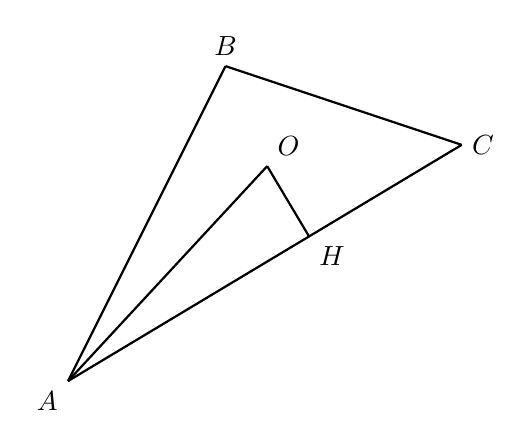
\begin{tikzpicture}
        \draw[-,thick] (0,0) node[anchor=north east]{$A$} -- (5,3) node[anchor=west]{$C$}
                       (5,3)                              -- (2,4) node[anchor=south]{$B$}
                       (2,4)                              -- (0,0);
        \draw[-,thick] (0,0)       -- (2.53,2.73) node[anchor=south west]{$O$}
                       (2.53,2.73) -- (3.06,1.84) node[anchor=north west]{$H$};
      \end{tikzpicture}
      
      \caption{Точка $O$ пересечения биссектрис $\triangle ABC$.}
      \label{fig:bisectors-intersection}
    \end{figure}
    
    Будем искать радиус вектор точки $O$ как $\vv O = \vv A + \vv{AO}$: положение $A$ известно, поэтому при таком пути решения надо получить $\vv{AO}$.

    \begin{figure}[h]
      \centering
      
      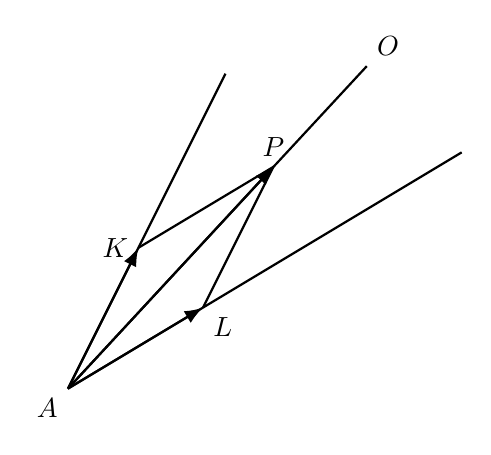
\begin{tikzpicture}
        \draw[-,thick] (0,0) node[anchor=north east]{$A$} -- (5,3)
                       (0,0)                              -- (2,4);
        \draw[-,thick]      (0,0)         -- (3.795,4.095) node[anchor=south west]{$O$};
        \draw[-Latex,thick] (0,0)         -- (1.714,1.028) node[anchor=north west]{$L$};  % (0.857,0.514)
        \draw[-,thick]      (1.714,1.028) -- (2.608,2.816) node[anchor=south]{$P$};       % (1.304,1.408)
        \draw[-Latex,thick] (0,0)         -- (0.894,1.788) node[anchor=east]{$K$};        % (0.447,0.894)
        \draw[-,thick]      (0.894,1.788) -- (2.608,2.816);
        \draw[-Latex,thick] (0,0)         -- (2.608,2.816);
      \end{tikzpicture}
      
      \caption{Вектор $\bds l \hm= \protect\vv{AP}$ в направлении прямой $AO$~---~сумма единичных векторов $\protect\vv{AK}$ и $\protect\vv{AL}$, направленных соответственно вдоль сторон $AB$ и $AC$ треугольника $ABC$.}
      \label{fig:l-parallel-ao}
    \end{figure}
    
    Начнём с того, что вектор в направлении прямой $AO$ (\ref{fig:l-parallel-ao}) можно получить как
    \begin{equation}\label{eq:l-vector}
      \bds l = \frac{\vv{AB}}{|AB|} + \frac{\vv{AC}}{|AC|}
    \end{equation}
    Но вектор не нормирован: $|\bds l| \hm{\not=} 1$.
    И сходу посчитать его модуль мы не можем (базис в задаче общий, не обязательно ортонормированный, поэтому скалярное произведение не выражается \emph{только} через компоненты векторов).
    Но модуль можно так выразить через угол $\alpha$ с помощью теоремы синусов для треугольника $APL$ (\ref{fig:l-parallel-ao}):
    \[
      \frac{AP}{\sin{\angle ALP}} = \frac{PL}{\sin{\angle PAL}}
    \]
    или, переходя к обозначениям $\bds l$ и $\alpha$ и пользуясь тем, что $|PL| \hm= 1$ по построению:
    \[
      \frac{|\bds l|}{\sin{(\pi - \alpha)}} = \frac{1}{\sin \frac{\alpha}{2}}
    \]
    В итоге получаем
    \begin{equation}\label{eq:l-module}
      |\bds l| = \frac{\sin \alpha}{\sin \frac{\alpha}{2}}
    \end{equation}
    
    Рассмотрим $\triangle AOH$ (\ref{fig:bisectors-intersection}).
    Сторона $AO$:
    \[
      AO = \frac{OH}{\sin \angle OAH} = \frac{r}{\sin \frac{\alpha}{2}}
    \]
    Вектор $\vv{AO}$:
    \[
      \vv{AO} = \frac{\bds l}{|\bds l|} \cdot |AO|
        \stackrel{(\ref{eq:l-module})}{=} \frac{\bds l}{\sin \alpha \Big/ \sin \frac{\alpha}{2}} \cdot \frac{r}{\sin \frac{\alpha}{2}}
        = \bds l \cdot \frac{r}{\sin \alpha}
        = \bigstar
    \]
    
    Радиус $r$ можно выразить через формулы для нахождения площади треугольника $\triangle ABC$:
    \[
      S_{\triangle ABC} = pr = \frac{1}{2} AC \cdot AB \cdot \sin \alpha
        \Rightarrow \frac{bc \sin \alpha}{2p}
    \]
    где $p$~---~полупериметр $\triangle ABC$, $b \hm\equiv AC$, $c \hm\equiv AB$.
    
    И тогда, возвращаясь к нахождению вектора $\vv{AO}$:
    \[
      \bigstar = \bds l \cdot \frac{r}{\sin \alpha}
        = \bds l \cdot \frac{bc}{2p}
        = \blacktriangledown
    \]
    
    Далее можно подставить вместо $\bds l$ его выражение через вектора $\vv{AC} \hm= \bds r_C \hm- \bds r_A$ и $\vv{AB} \hm= \bds r_B \hm- \bds r_A$ (\ref{eq:l-vector}) и вместо $p$ его выражение через длины сторон $\triangle ABC$ ($BC \hm\equiv a$):
    \[
      \blacktriangledown = \left(\frac{\bds r_C - \bds r_A}{b} + \frac{\bds r_B - \bds r_A}{c}\right) \cdot \frac{bc}{a + b + c}
        = \frac{c(\bds r_C - \bds r_A) + b(\bds r_B - \bds r_A)}{a + b + c}
    \]
    
    И в итоге для радиуса-вектора центра вписанной окружности $O$ получаем выражение:
    \[
      \bds r_O = \bds r_A + \vv{AO}
        = \frac{a \bds r_A + b \bds r_B + c \bds r_C}{a + b + c}
        = \frac{|\bds r_C - \bds r_B| \bds r_A + |\bds r_C - \bds r_A| \bds r_B + |\bds r_A - \bds r_B| \bds r_C}{|\bds r_C - \bds r_B| + |\bds r_C - \bds r_A| + |\bds r_A - \bds r_B|}
    \]
  \end{solution}
  
  
  \section{Дополнение}
  
  \subsection{Про центр масс}
  
  Есть задача, где надо было найти центр масс однородной проволоки, изогнутой под углом.
  В общем случае положение центра масс тела объёма $V$ и массы $M$ вычисляется по формуле
  \[
    \bds r_c = \frac{1}{M} \int_V \rho(\bds r) \bds r dV
  \]
  где $\rho(\bds r)$~---~плотность в точке $\bds r$.
  
  Поэтому, даже в случае, когда система состоит не из материальных точек, а из протяжённых тел, центр масс системы тоже можно вычислять как взвешенное среднее центров масс отдельных частей (потому что интеграл по телу разбивается на несколько интегралов).
  
  В задаче же про центр масс треугольника не важно, где сосредоточена масса в треугольнике: в вершинах или распределена равномерно по сторонам.
  \sout{Положение центра масс в обоих случаях будет одинаковое.}
  Положение центра масс в случае распределения массы по сторонам будет таким же, как и в случае, когда массы сосредоточены в вершинах, если все стороны одинаковой массы (то есть плотность на разных сторонах может быть разной).
  Если же масса пропорциональна длине стороны (например, плотность одинакова по сторонам), то центр масс будет смещён к более длинной стороне.
\end{document}